\section{Experiments}

In this section, we conduct experiments to address the following research questions:

\begin{itemize}
    \item \textbf{RQ1: }Does a global semantic structure exist within the latent space?
    \item \textbf{RQ2: }What type of latent space is optimal for text generation?
    \item \textbf{RQ3: }Which diffusion process is most effective for text generation?
    \item \textbf{RQ4: }Why use a \emph{continuous} \emph{latent} \emph{diffusion} model for language modeling?
\end{itemize}

\subsection{Experimental Setup}

\textbf{Datasets. }
For training, we use external open-source pretraining data. For evaluation, the internal component analysis of \method (Sections~\ref{exp:rq1}, \ref{exp:rq2} and \ref{exp:rq3}) is conducted on randomly sampled subsets from the test sets of LAMBADA \citep{paperno2016lambada}, MMLU \citep{hendrycks2020measuring}, and SIQA \citep{sap2019social}. LAMBADA is a continuation benchmark, whereas the remaining two are multiple-choice benchmarks. For external comparisons (Section~\ref{exp:rq4}), we additionally evaluate on the test sets of SQuAD \citep{rajpurkar2016squad}, Story Cloze \citep{mostafazadeh2016corpus}, OBQA \citep{mihaylov2018can}, RACE \citep{lai2017race}, and HellaSwag \citep{zellers2019hellaswag}. Additional dataset details are deferred to Appendix~\ref{app:dataset}.

\textbf{Baselines. } 
In the internal component comparison experiments (Sections~\ref{exp:rq1}, \ref{exp:rq2} and \ref{exp:rq3}), we specify the different configurations of \method. In Section~\ref{exp:rq4}, for the scaling comparison, we independently train the autoregressive and LLaDA baselines under strictly matched settings. Specifically, the autoregressive and discrete diffusion models are randomly initialized using the official modeling implementations of LLaMA \citep{touvron2023llama} and LLaDA \citep{nie2025large}, respectively. Details are provided in Appendix~\ref{app:baseline}.

\textbf{Metrics. }
As discussed in Section~\ref{dis:ppl}, the estimated perplexity exhibits a substantial mismatch with the actual generation quality of \method. Moreover, prior work \citep{wang2023knn, hashimoto2019unifying, holtzman2019curious, meister2021language} has noted that perplexity is not strictly correlated with generation performance. To enable the most objective and fair comparison, we therefore evaluate all models under a unified few-shot setting across both multiple-choice and generative tasks. For multiple-choice benchmarks and continuation tasks such as Lambada and SQuAD, accuracy is computed by strict string matching between the model output and the ground-truth answer under predefined rules. Additional evaluation details are provided in Appendix~\ref{app:metrics}.

\textbf{Setup. }
\method uses the OLMo 2 \citep{olmo20242} tokenizer and is trained with AdamW. The learning rate starts at \(1\times10^{-6}\), is linearly warmed up to \(1.5\times10^{-4}\) over the first 5{,}000 steps, and is then decayed with a cosine schedule to \(1\times10^{-5}\) by 1{,}000{,}000 steps. All evaluations are conducted using the checkpoint at the corresponding FLOPs budget, without EMA weights. The same tokenizer, optimization and evaluation settings are used for \method and all external baselines. In \method, the VAE contains 500M parameters and the DiT contains 1.8B parameters. For the autoregressive and discrete diffusion baselines, the embedding layer has approximately 400M parameters and the non-embedding backbone has 1.8B parameters. We thus keep the total model size of the two model families at a comparable scale of roughly 2B parameters. All methods are trained with the same random seed so that the training data are matched across runs, with the maximum sequence length set to 512. Additional details are provided in Appendix~\ref{app:setup} and~\ref{app:fairness_embed_vae_latent_space}.

\subsection{Evidence of Global Semantic Structures in Cola DLM (RQ1)}
\label{exp:rq1}
In this section, we first present an implication for the existence of global semantic structures, and then provide strong empirical evidence for their existence by quantitatively examining the performance of latent spaces with different dimensions under different timestep shifts. The full theoretical derivation, proof, and technical details are provided in Appendix~\ref{sec:global_semantic_structure}.

\implicationbox{imp:rq1_global_semantic_structure}{
If the latent representation is purely local and fully separable, then the optimal timeshift does not exhibit a stable drift as the latent dimension changes. Therefore, if the optimal timeshift is observed to shift systematically with the latent dimension in experiments, this indicates the existence of cross-dimensional shared structures in the latent space; if this phenomenon is mainly reflected in semantic metrics, it further supports that these shared structures are related to high-level semantics.
}

Based on Implication~\ref{imp:rq1_global_semantic_structure}, the focus of this section is not merely on the specific optimal loc values under different latent dimensions, but on whether the peak position of the optimal timeshift exhibits a stable and regular shift as the latent dimension varies. Figure~\ref{fig:rq1_global_semantic_structure} presents the corresponding experimental results.

\textbf{Obs. \ding{182} The optimal timeshift exhibits a systematic drift with the latent dimension. }As shown in the left panel of Figure~\ref{fig:rq1_global_semantic_structure}, the best loc for Task Avg shifts from approximately $1.0$ at $d=16$, to approximately $1.7$ at $d=64$, and further to approximately $2.3$ at $d=128$. This trend is clear and approximately monotonic. This phenomenon directly contradicts the separable null hypothesis. A more plausible explanation is that changing the latent dimension alters the effective noise calibration position of some cross-dimensional shared structure.

\textbf{Obs. \ding{183} This trend is consistent across multiple semantic metrics. }The right panel of Figure~\ref{fig:rq1_global_semantic_structure} further shows that, although the best loc values for LAMBADA, MMLU, SIQA, and Task Avg are not exactly the same, they all overall favor larger loc regions as the latent dimension increases. This indicates that the peak drift is not an accidental fluctuation of any single task, but rather a stable phenomenon jointly supported by multiple semantic evaluations. Therefore, what is modulated by timeshift is a representation structure shared across different semantic tasks.

\textbf{Obs. \ding{184} The empirical peaks are broadly consistent with the theoretical predictions. }In the left panel of Figure~\ref{fig:rq1_global_semantic_structure}, the dashed lines indicate the theoretically predicted optimal loc values. It can be seen that, under all three latent-dimension settings, the empirical peaks are close to the predicted positions, and the drift directions are fully consistent. This suggests that the observed drift is not an arbitrary empirical hyperparameter effect, but is instead consistent with the theoretical analysis in Appendix~\ref{sec:global_semantic_structure}, namely that shared latent structures lead to dimension-dependent timeshift calibration.

Implication~\ref{imp:rq1_global_semantic_structure} provides a rigorous contrapositive statement for the existence of global semantic structures, while the experimental results, by providing reverse evidence for this contrapositive, offer strong empirical support for the existence of shared and semantically relevant global structures in the latent space of \method. This also provides supporting evidence for the first condition in Eq.~\eqref{eq:main_three_curves} of Section~\ref{sec:theory_advantage}, thereby further supporting the advantage of \method.

\begin{figure}[t]
    \centering
    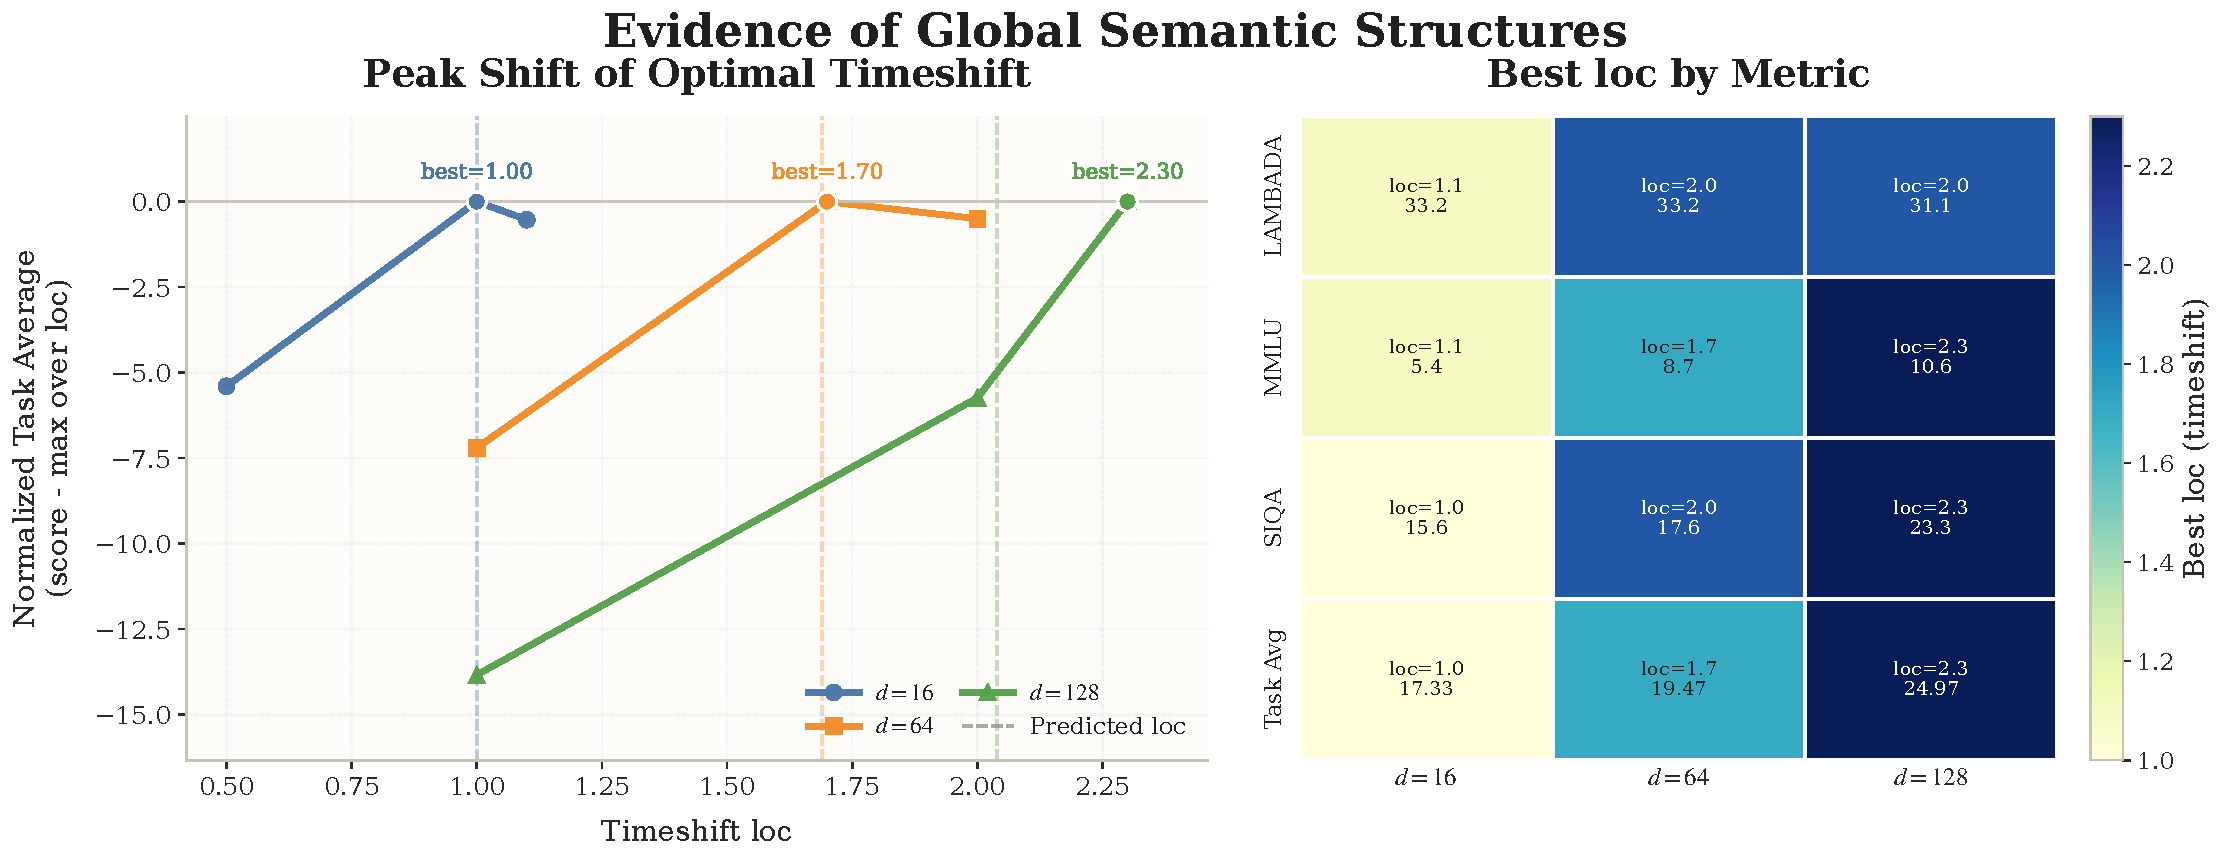
\includegraphics[width=\textwidth]{exp_fig/rq1/global_semantic_structure_evidence.pdf}
    \caption{\textbf{Evidence of global semantic structures in the latent space.} Left: as latent dimension increases, optimal timeshifts move toward larger locations, with empirical peaks matching predictions. Right: most of the evaluation metrics consistently prefer larger best locations at higher dimensions. This stable cross-metric trend supports shared global semantic structures within the latent space.}
    \label{fig:rq1_global_semantic_structure}
\end{figure}

\subsection{Analysis of Different Latent Spaces in Cola DLM (RQ2)}
\label{exp:rq2}

In this section, we present a detailed empirical study of different latent spaces through both quantitative evaluation and visualization. We analyze the design of the latent space from three perspectives: whether it should be dynamic or static, what latent dimensionality is most appropriate, and how semantic smoothness contributes to latent-space quality. Based on these analyses, we identify the most effective directions for optimizing the latent space.

\begin{figure}[t]
    \centering
    \begin{subfigure}[t]{0.49\linewidth}
        \centering
        
\includegraphics[width=\linewidth]{exp_fig/rq2/fix_vs_evolve/line/tasks_avg.pdf}
        \label{fig:rq2_fix_vs_evolve_tasks_avg}
    \end{subfigure}
    \hfill
    \begin{subfigure}[t]{0.49\linewidth}
        \centering
        
\includegraphics[width=\linewidth]{exp_fig/rq2/fix_vs_evolve/line/lambada.pdf}
        \label{fig:rq2_fix_vs_evolve_lambada}
    \end{subfigure}

    \vspace{0.5em}

    \begin{subfigure}[t]{0.49\linewidth}
        \centering
        
\includegraphics[width=\linewidth]{exp_fig/rq2/fix_vs_evolve/line/mmlu.pdf}
        \label{fig:rq2_fix_vs_evolve_mmlu}
    \end{subfigure}
    \hfill
    \begin{subfigure}[t]{0.49\linewidth}
        \centering
        
\includegraphics[width=\linewidth]{exp_fig/rq2/fix_vs_evolve/line/siqa.pdf}
        \label{fig:rq2_fix_vs_evolve_siqa}
    \end{subfigure}
    \caption{\textbf{Comparison between fixed and evolving latent spaces.} Across Task Average, LAMBADA, MMLU, and SIQA, joint evolution with DiT achieves the best overall scaling and performance when initialized from a stable pretrained VAE. Fixed spaces lead to earlier saturation, while training from scratch or interval updates remains less effective. This suggests the space should evolve with DiT, but from a stable initialization rather than scratch.}
    \label{fig:rq2_fix_vs_evolve}
\end{figure}

\begin{figure}[t]
    \centering
    \begin{subfigure}[t]{0.32\linewidth}
        \centering
        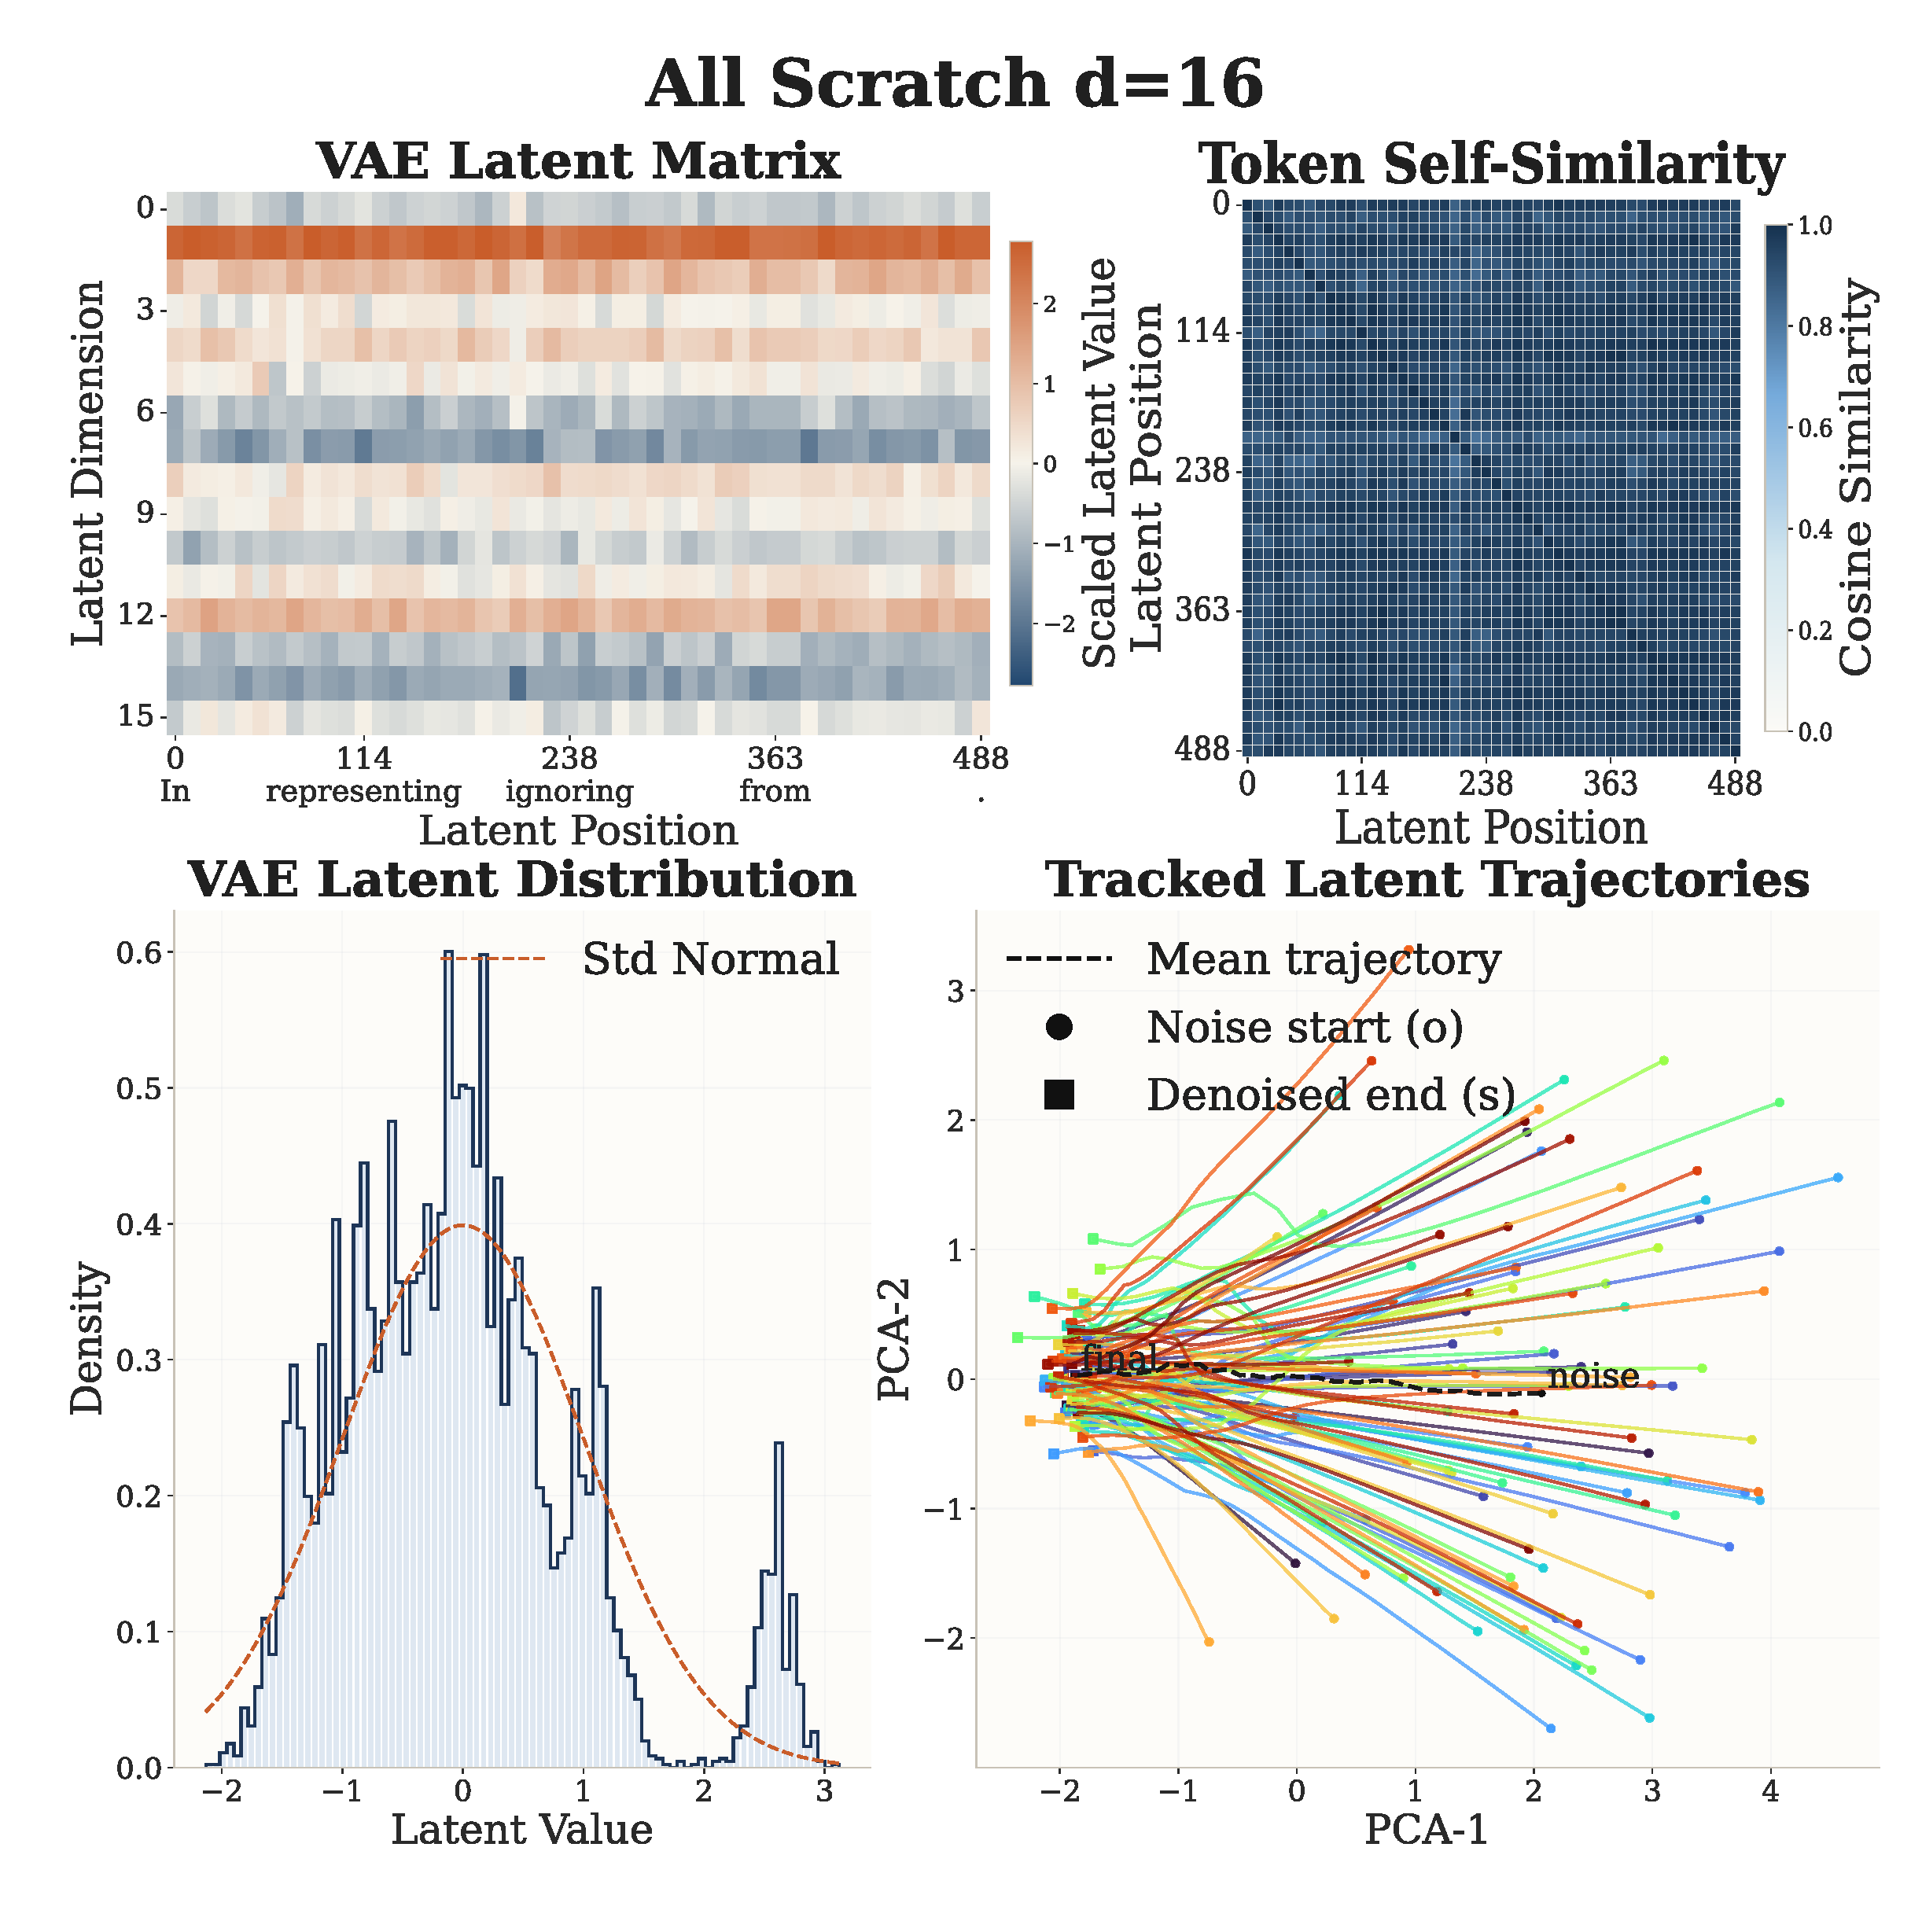
\includegraphics[width=\linewidth]{exp_fig/rq2/fix_vs_evolve/visualize/all_sc_16.pdf}
        \label{fig:rq2_fix_vs_evolve_vis_all_sc_16}
    \end{subfigure}
    \hfill
    \begin{subfigure}[t]{0.32\linewidth}
        \centering
        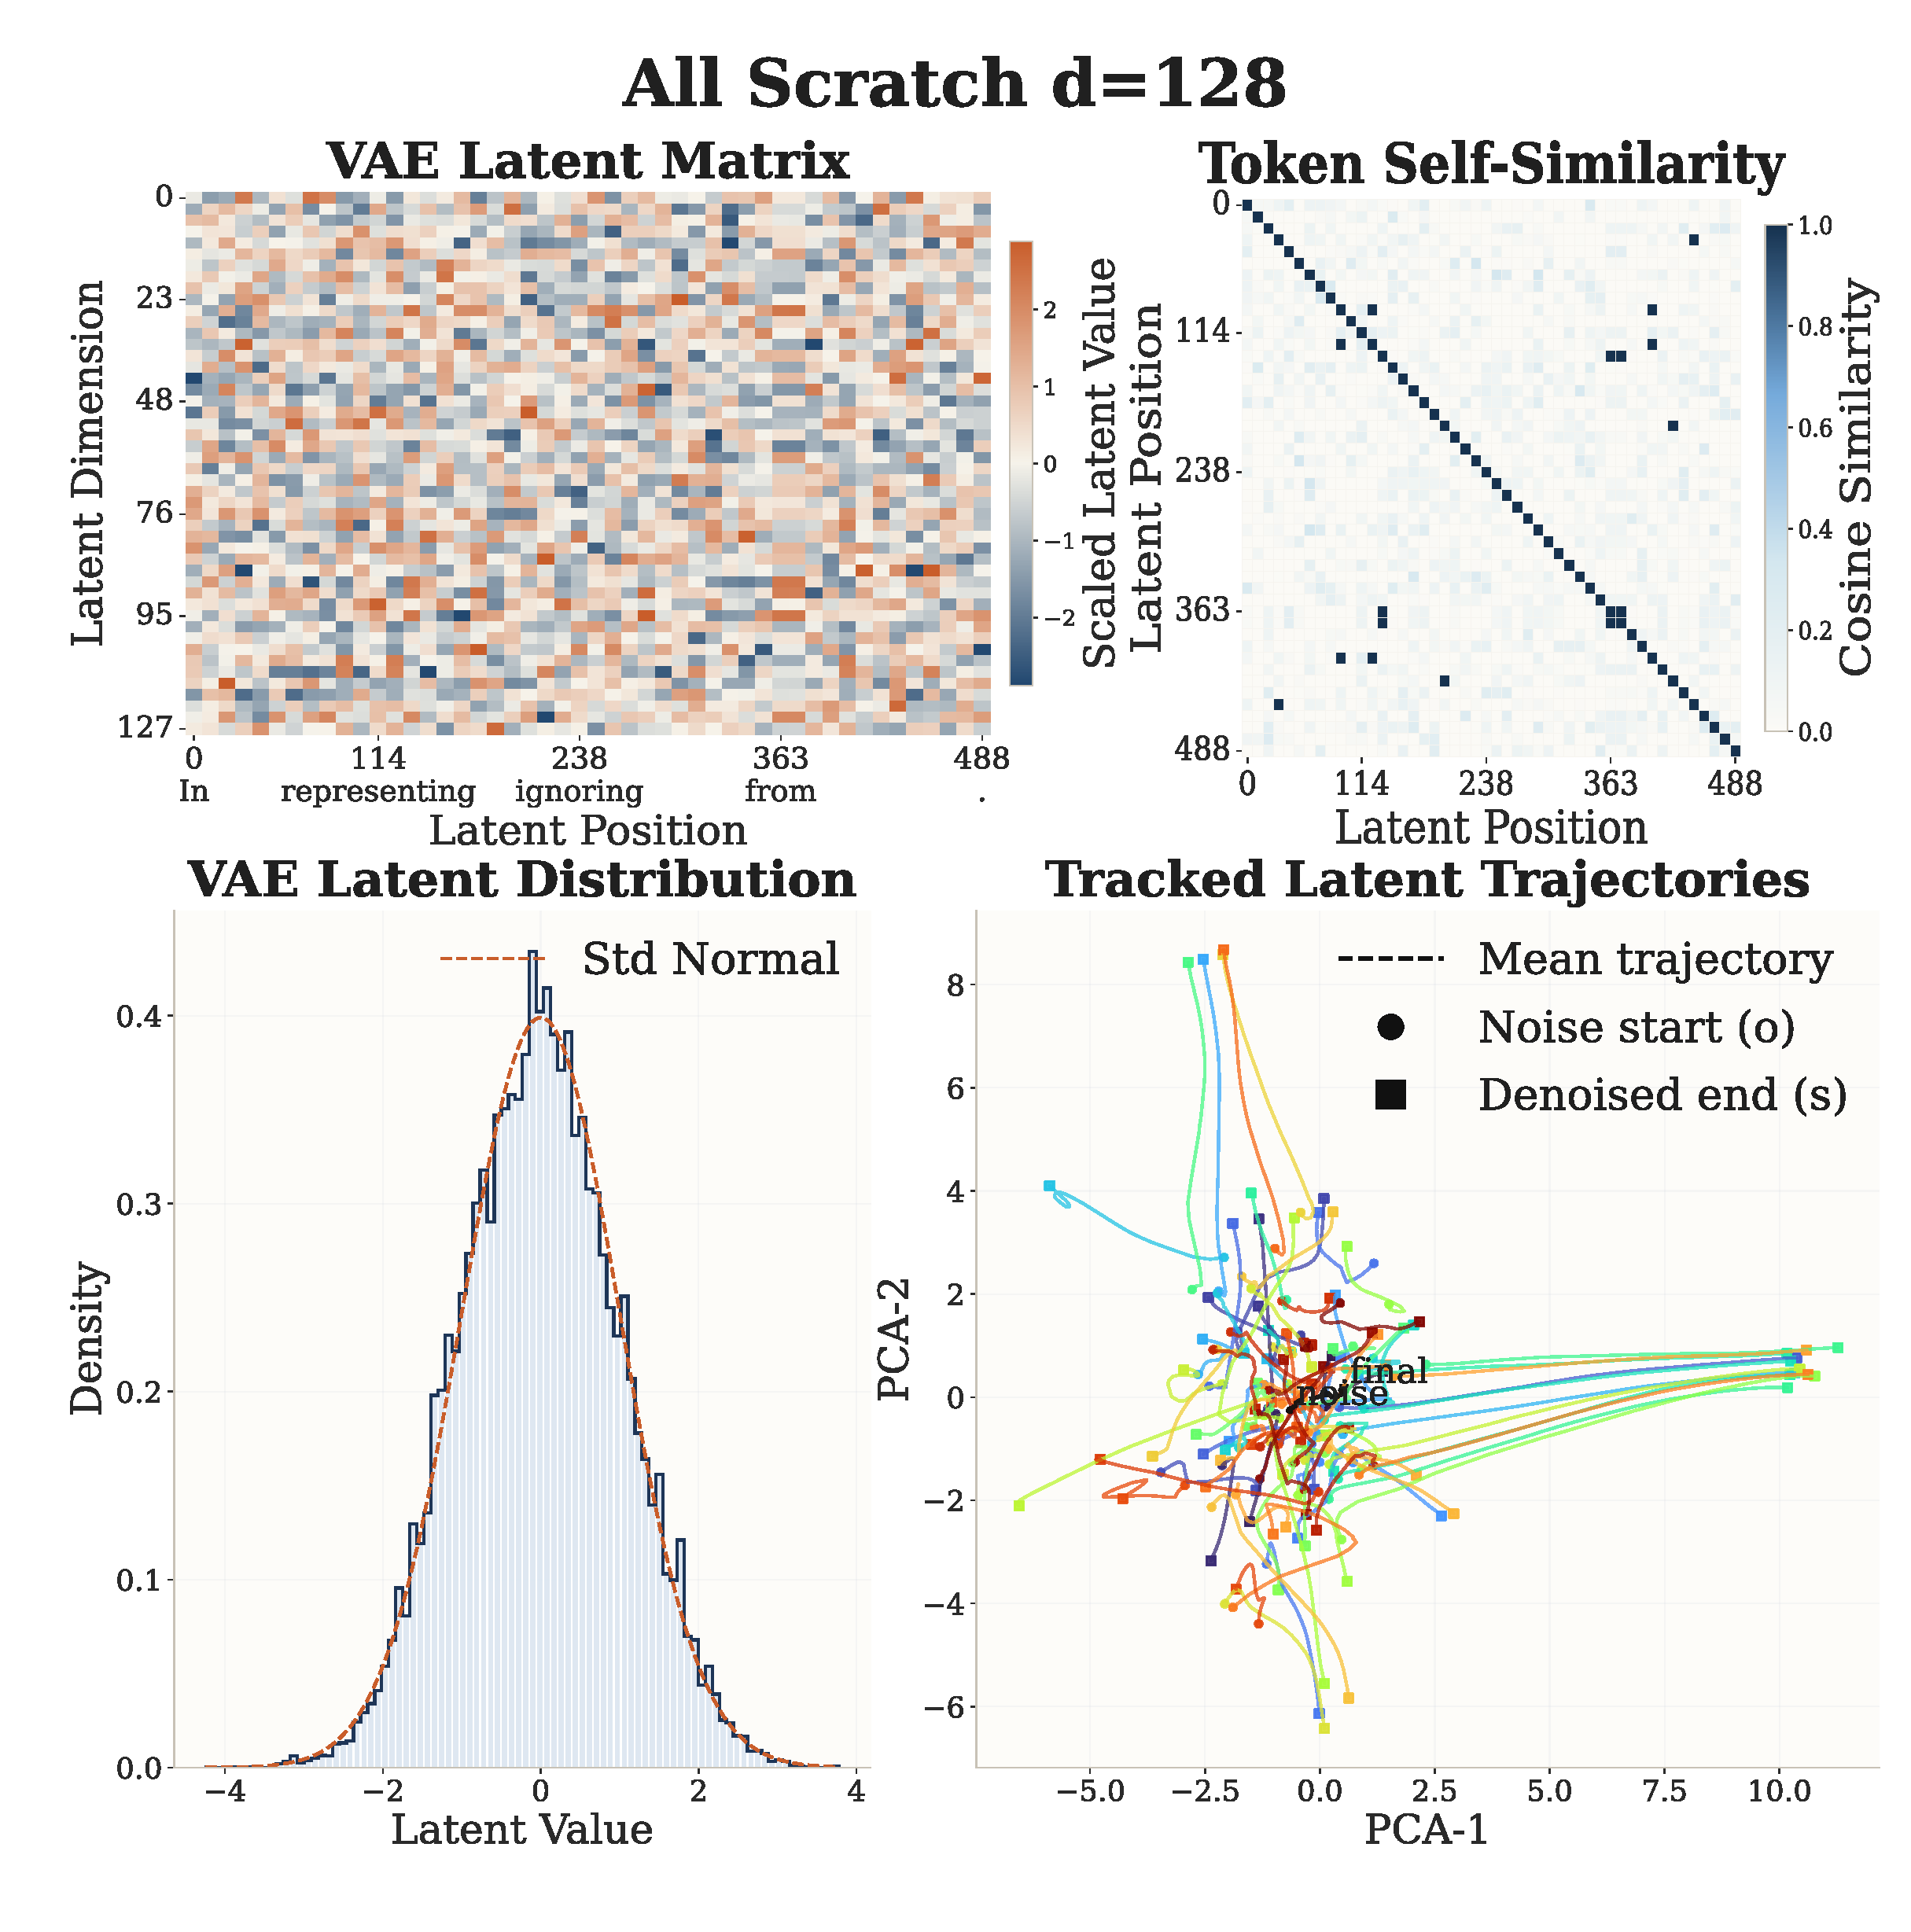
\includegraphics[width=\linewidth]{exp_fig/rq2/fix_vs_evolve/visualize/all_sc_128.pdf}
        \label{fig:rq2_fix_vs_evolve_vis_all_sc_128}
    \end{subfigure}
    \hfill
    \begin{subfigure}[t]{0.32\linewidth}
        \centering
        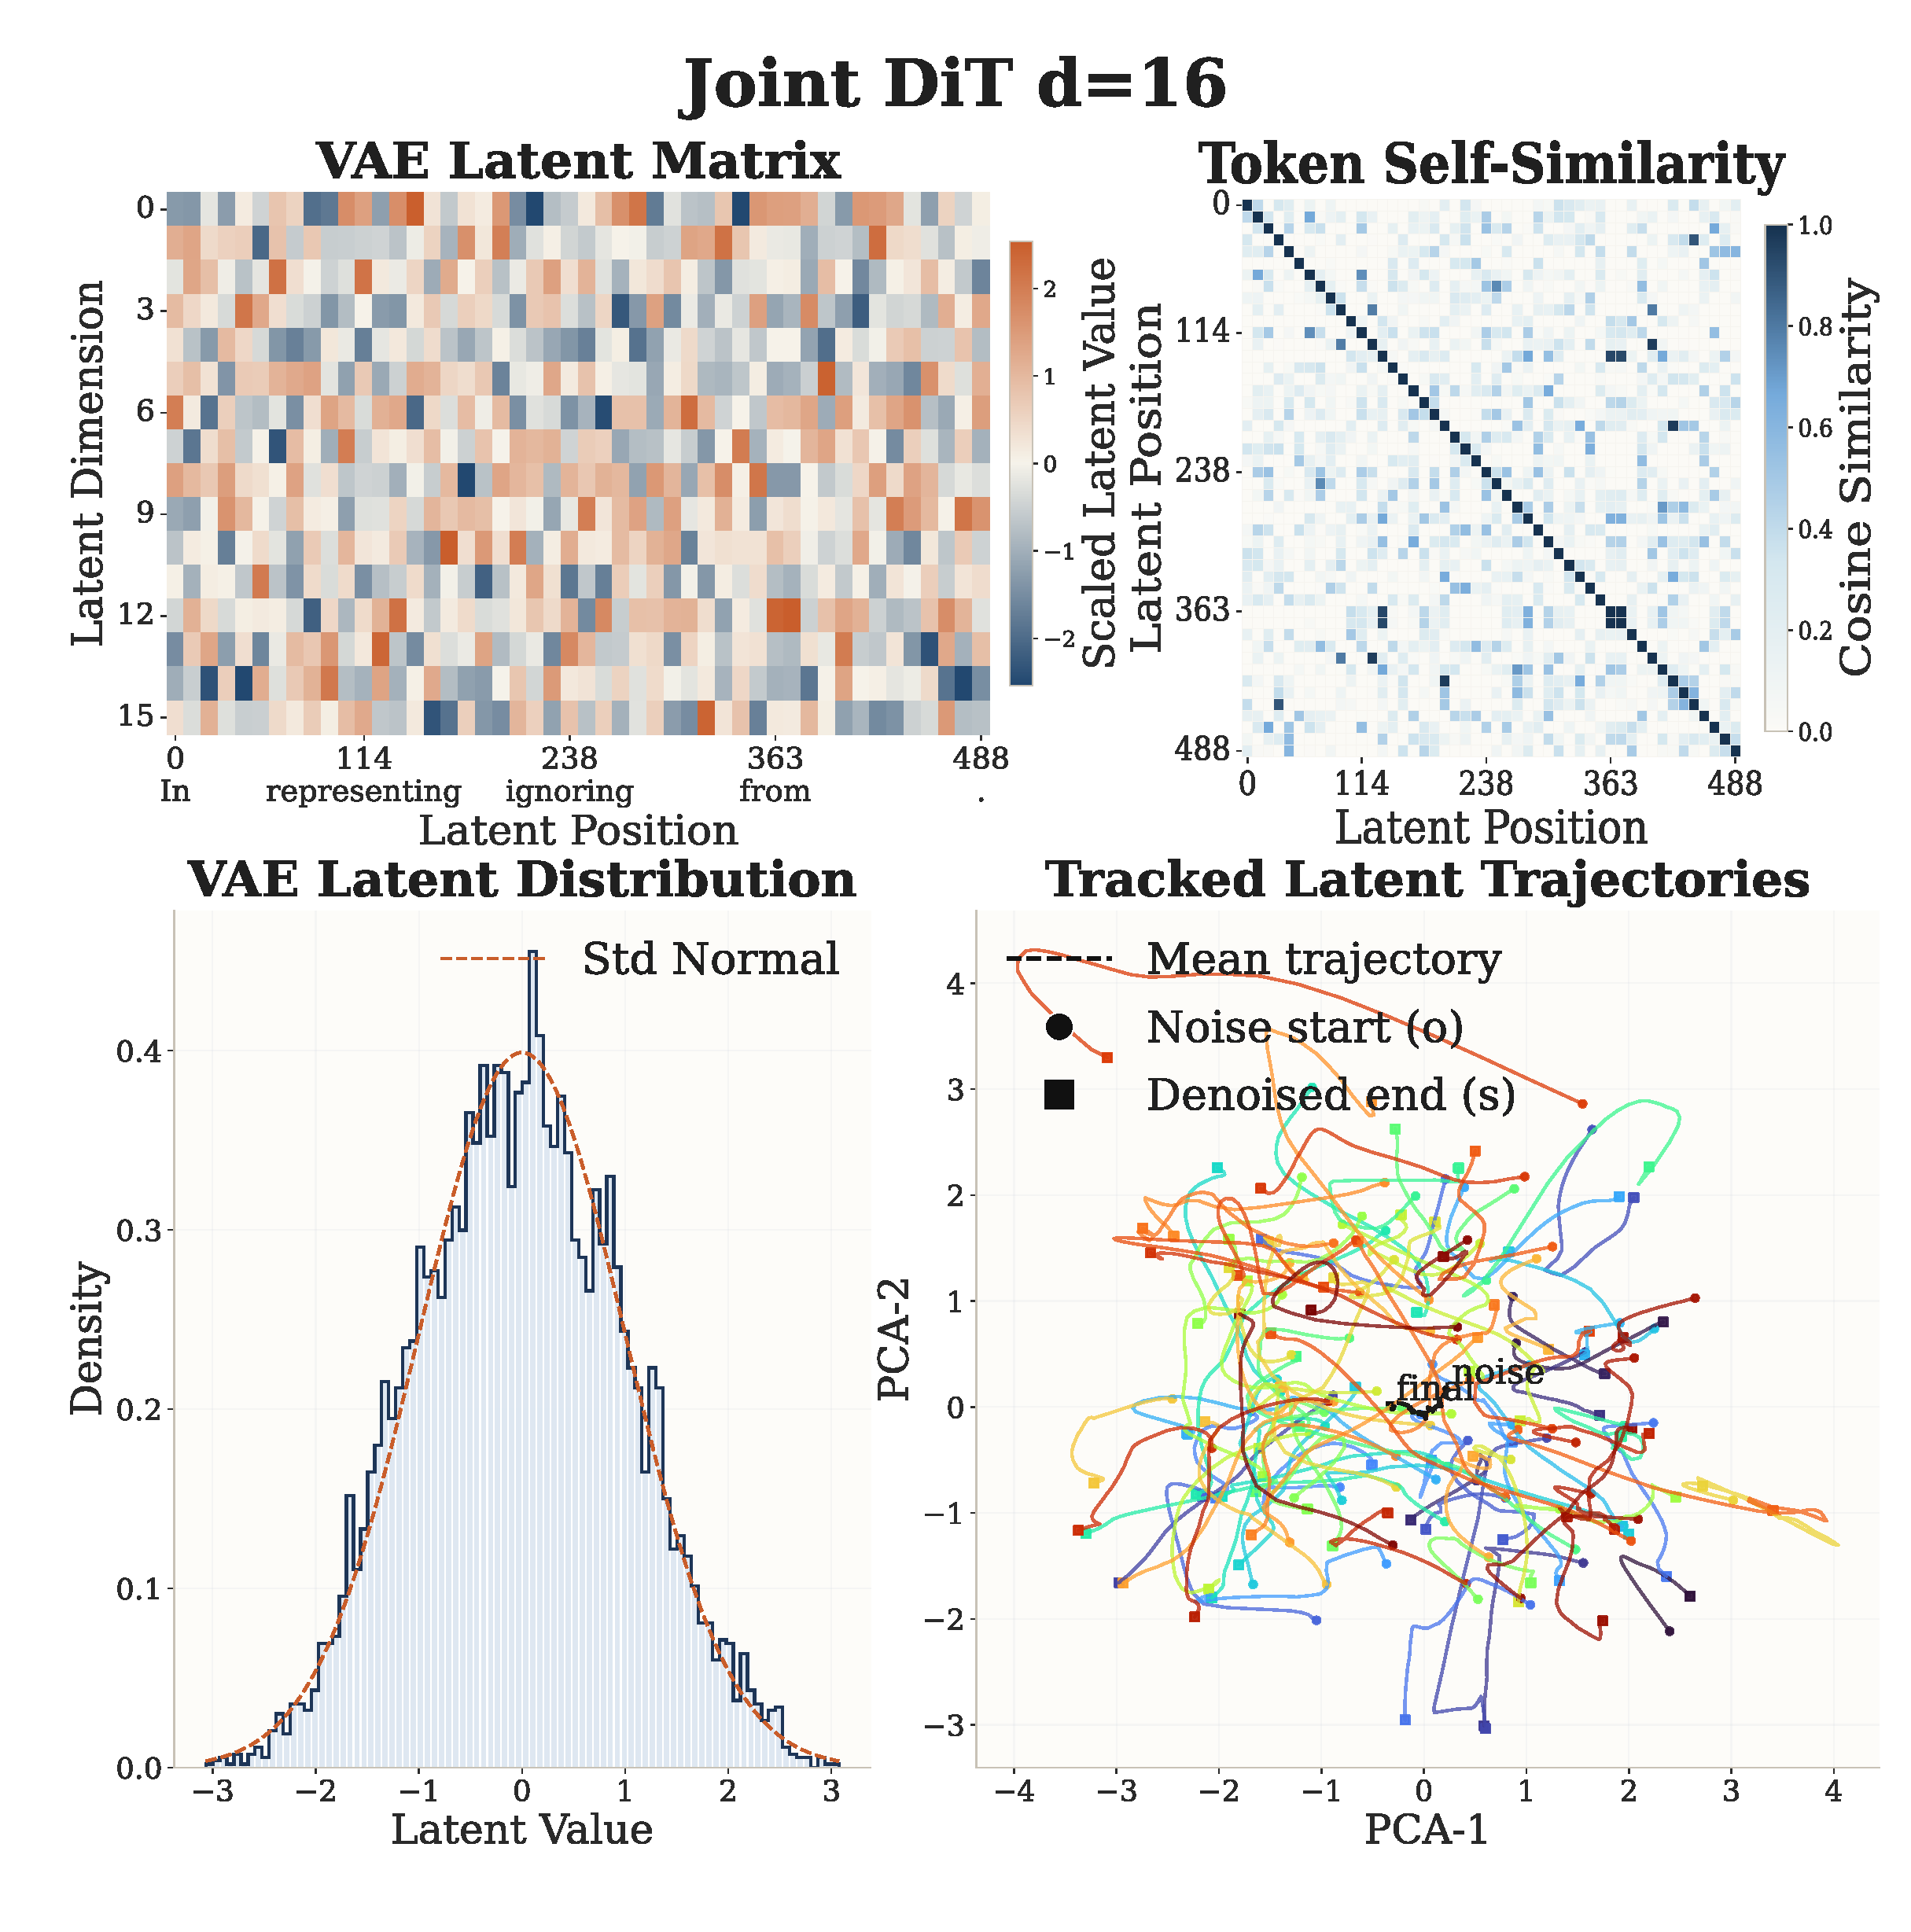
\includegraphics[width=\linewidth]{exp_fig/rq2/fix_vs_evolve/visualize/dit_sc_16.pdf}
        \label{fig:rq2_fix_vs_evolve_vis_dit_sc_16}
    \end{subfigure}
    \caption{\textbf{Visualization of latent spaces under different training strategies.} Joint optimization on a stable initialization yields a more structured, semantically organized latent space than training VAE and DiT from scratch. Increasing the latent dimension ($16$ to $128$) partially mitigates collapse but remains less structured than the stable-initialization approach.}
    \label{fig:rq2_fix_vs_evolve_visualize}
\end{figure}

\paragraph{Fixed vs. Evolving Latent Space.}
As shown in Figure~\ref{fig:rq2_fix_vs_evolve}, this section studies whether the latent space should evolve jointly with DiT during training. Under the same compute budget, we compare five strategies: fixing a pretrained VAE (Fix VAE); initializing the VAE from pretrained weights and jointly training it with DiT using a VAE learning rate equal to that of DiT or scaled to $0.01\times$ (Joint DiT x1 / Joint DiT x0.01); jointly training both VAE and DiT from random initialization with the same learning rate (All Scratch x1); and an interval-based strategy (Interval), where each $5$k-step cycle consists of $2$k steps of joint training followed by $3$k steps with the VAE frozen. The overall results suggest that the latent space should neither remain fully fixed nor be jointly optimized from scratch without constraint. Instead, the most effective strategy is to let it evolve together with DiT on top of a stable initialization.

\textbf{Obs. \ding{182} Joint DiT x1 shows the strongest scaling potential.}
At small compute budgets, Fix VAE and Joint DiT x1 are close, and Fix VAE is sometimes slightly better. As FLOPs increase, however, Joint DiT x1 improves more steadily and achieves the best final results on Task Avg, LAMBADA, MMLU, and SIQA, whereas Fix VAE gradually saturates. This indicates that a fixed latent space helps early stability but limits the performance ceiling, while continuous co-adaptation with DiT is more beneficial for scaling.

\textbf{Obs. \ding{183} The benefit of joint training depends on good initialization rather than trainability alone.}
All Scratch x1 performs consistently worse than the other methods across all metrics, and its gains remain limited throughout training. This suggests that the advantage of Joint DiT x1 does not come from making the latent space trainable by itself; it relies on starting from a meaningful pretrained latent space and then adapting it jointly with DiT.

\textbf{Obs. \ding{184} The latent-space visualization explains why All Scratch underperforms.}
Figure~\ref{fig:rq2_fix_vs_evolve_visualize} shows that All Scratch with $d=16$ yields a more collapsed and less structured latent space, with trajectories dominated by simple outward drift. Increasing the latent dimension to $128$ partially alleviates this issue, but the geometry still remains less organized than that of Joint DiT with stable initialization. In contrast, Joint DiT produces more heterogeneous latent patterns and richer trajectories, suggesting a more structured and semantically usable space.

\textbf{Obs. \ding{185} Effective latent evolution requires both continuous participation and sufficient update strength.}
Joint DiT x0.01 and Interval are both better than All Scratch x1, but still clearly worse than Joint DiT x1 in overall trend and final performance. This shows that partial latent participation is not enough: overly weak updates slow adaptation, while periodic freezing disrupts co-evolution with DiT. A better strategy is to update the latent space continuously and strongly, while keeping the initialization stable.

Overall, Figure~\ref{fig:rq2_fix_vs_evolve} and Figure~\ref{fig:rq2_fix_vs_evolve_visualize} consistently show that the best latent-space strategy is neither to keep it fixed nor to train it from scratch, but to let it evolve jointly with DiT on top of a good initialization. When the VAE and DiT are trained jointly, the VAE is exposed to more data and can fit $\pdata(z|x)$ more accurately. This further verifies the last condition in Eq.~\eqref{eq:main_three_curves} of Section~\ref{sec:theory_advantage}, and provides strong support for the potential advantage of \method. Additional results are in Appendix~\ref{app:fix_vs_evolve_fulu}.

\begin{wraptable}{r}{0.55\textwidth}
    \vspace{-0.8em}
    \centering
    \caption{\textbf{Dimensionality of the latent space under 117 EFLOPs.} Larger latent dimensions improve the overall average under the all-scratch setting with $\mathrm{loc}=1$.}
    \label{tab:latent_dim_half}
    \small
    \setlength{\tabcolsep}{3.5pt}
    \renewcommand{\arraystretch}{1.08}
    \begin{tabular}{lcccc}
        \toprule
        Method & Lambada & MMLU & SIQA & Avg. \\
        \midrule
        All Scratch, $d=16$, loc=1  & 14.3 & \underline{6.9} & 4.9 & 8.7 \\
        All Scratch, $d=64$, loc=1  & \textbf{20.9} & 5.4 & \underline{7.6} & \underline{11.3} \\
        All Scratch, $d=128$, loc=1 & \underline{18.5} & \textbf{8.1} & \textbf{8.9} & \textbf{11.8} \\
        \bottomrule
    \end{tabular}
    \vspace{-0.8em}
\end{wraptable}

\paragraph{Dimensionality of the Latent Space. }
We next study how the latent dimensionality affects both performance and latent-space quality. Table~\ref{tab:latent_dim_half} compares All Scratch models with different latent dimensions under the same EFLOPs budget ($117$), Figure~\ref{fig:rq2_fix_vs_evolve_visualize} provides the corresponding latent-space visualization, and Figure~\ref{fig:rq1_global_semantic_structure} shows how the optimal timeshift changes with dimension. Taken together, these results suggest that increasing the latent dimension partially alleviates collapse and improves semantic capacity, but it also changes the effective noise calibration of the latent space.

\textbf{Obs. \ding{182} Increasing the latent dimension improves the overall semantic capacity under the same compute budget.}
As shown in Table~\ref{tab:latent_dim_half}, the average score increases from $8.7$ at $d=16$ to $11.3$ at $d=64$, and further to $11.8$ at $d=128$. The improvement is most evident on MMLU and SIQA. Although LAMBADA peaks at $d=64$, the overall trend still suggests that a larger latent space carries stronger semantic capacity under the same compute budget.

\textbf{Obs. \ding{183} A larger latent dimension partially alleviates latent-space collapse, but does not fully solve it.}
Figure~\ref{fig:rq2_fix_vs_evolve_visualize} shows that increasing the dimension from $16$ to $128$ makes the latent space less collapsed and more dispersed. However, the resulting geometry still remains clearly less structured than Joint DiT with stable initialization. This indicates that increasing dimensionality is helpful, but cannot by itself replace proper latent-space formation.

\begin{figure}[t]
    \centering
    \begin{subfigure}[t]{0.49\linewidth}
        \centering
        
\includegraphics[width=\linewidth]{exp_fig/rq2/semantic/tasks_avg.pdf}
        \label{fig:rq2_semantic_tasks_avg}
    \end{subfigure}
    \hfill
    \begin{subfigure}[t]{0.49\linewidth}
        \centering
        
\includegraphics[width=\linewidth]{exp_fig/rq2/semantic/lambada.pdf}
        \label{fig:rq2_semantic_lambada}
    \end{subfigure}

    \vspace{0.5em}

    \begin{subfigure}[t]{0.49\linewidth}
        \centering
        
\includegraphics[width=\linewidth]{exp_fig/rq2/semantic/mmlu.pdf}
        \label{fig:rq2_semantic_mmlu}
    \end{subfigure}
    \hfill
    \begin{subfigure}[t]{0.49\linewidth}
        \centering
        
\includegraphics[width=\linewidth]{exp_fig/rq2/semantic/siqa.pdf}
        \label{fig:rq2_semantic_siqa}
    \end{subfigure}
    \caption{\textbf{Effect of semantic smoothness in the latent space under the Joint DiT setting.} Adding a BERT-style loss consistently improves performance, with larger gains during active latent updates ($\mathrm{lr}=1$). This suggests semantic smoothness benefits latent-space quality, especially when evolving jointly with DiT.}
    \label{fig:rq2_semantic_importance}
\end{figure}

\textbf{Obs. \ding{184} The effect of latent dimensionality is not only geometric, but also dynamical.}
Figure~\ref{fig:rq1_global_semantic_structure} shows that the best timeshift systematically shifts toward larger loc values as the latent dimension increases. This means that increasing the latent dimension does not merely enlarge the space; it also changes the denoising scale at which semantic information is best recovered. Therefore, the benefit of a higher-dimensional latent space depends not only on improved geometry, but also on proper noise calibration.

Overall, Table~\ref{tab:latent_dim_half}, Figure~\ref{fig:rq2_fix_vs_evolve_visualize}, and Figure~\ref{fig:rq1_global_semantic_structure} present a consistent picture: increasing the latent dimension improves latent-space quality and downstream performance, but the gain is only partial, and its full benefit still depends on proper training dynamics and timeshift calibration.

\paragraph{Semantic Importance of the Latent Space. }
As shown in Figure~\ref{fig:rq2_semantic_importance}, all results in this subsection are obtained under the Joint DiT setting, where the VAE is initialized from pretrained weights and jointly optimized with DiT. We further compare whether to add a BERT-style loss in VAE training, which encourages the latent space to preserve smoother local semantics. Here, the reported lr denotes the VAE learning-rate ratio relative to DiT. The results show that such semantic smoothness is important for downstream performance, especially when the latent space is allowed to evolve more actively.

\textbf{Obs. \ding{182} Adding BERT loss consistently improves performance when the latent space is actively updated.}
When the VAE learning-rate ratio is $1$, BERT loss gives the best overall results across nearly the entire training range. In Figure~\ref{fig:rq2_semantic_importance}, the BERT-loss curve consistently outperforms its no-BERT counterpart on Task Average, LAMBADA, MMLU, and SIQA, and also achieves the best final performance. This indicates that encouraging masked-token recoverability makes the latent space more semantically useful for downstream prediction.

\textbf{Obs. \ding{183} Strong latent evolution is effective only with semantic guidance.}
When the VAE learning-rate ratio is $0.01$, adding BERT loss brings only limited gains, whereas its advantage becomes clear and stable when the ratio is increased to $1$. At the same time, simply increasing the VAE update strength without BERT loss does not reliably improve performance and is even weaker at several later-stage points. This shows that trainability alone is not sufficient: when the latent space evolves more actively, its updates must also be constrained toward a semantically smoother organization.

Overall, Figure~\ref{fig:rq2_semantic_importance} shows that semantic smoothness is an important property of a useful latent space. It not only improves final performance, but also makes joint latent evolution substantially more effective and stable. These results suggest that the latent should be compact but semantically sufficient, consistent with Eq.~\eqref{eq:main_avg_elbo} and Eq.~\eqref{eq:main_three_curves}. The BERT-style loss helps retain useful semantics under the bottleneck.

\begin{table}[t]
    \centering
    \caption{\textbf{Performance under different VAE logSNR settings.} VAE logSNR strongly affects downstream performance. A learnable setting gives the best overall results, while fixed logSNR = 1.5 is the strongest fixed alternative.}
    \label{tab:fixlogsnr_two_budgets}
    \small
    \setlength{\tabcolsep}{5pt}
    \renewcommand{\arraystretch}{1.10}
    \begin{tabular*}{\textwidth}{@{\extracolsep{\fill}}lcccc@{\hspace{1.2em}}cccc}
        \toprule
        \textbf{Compute Budget}
        & \multicolumn{4}{c}{\textbf{EFLOPs = 77.86}}
        & \multicolumn{4}{c}{\textbf{EFLOPs = 116.78}} \\
        \cmidrule(r){1-1} \cmidrule(lr){2-5} \cmidrule(lr){6-9}
        \textbf{Method}
        & \textbf{Lambada} & \textbf{MMLU} & \textbf{SIQA} & \textbf{Avg.}
        & \textbf{Lambada} & \textbf{MMLU} & \textbf{SIQA} & \textbf{Avg.} \\
        \midrule
        Fixed VAE logSNR = 1.0 & 27.1 & 5.7 & 11.3 & 14.70 & 30.4 & 7.7 & 18.4 & 18.83 \\
        Fixed VAE logSNR = 1.5 & 29.5 & \underline{7.8} & \textbf{17.5} & \underline{18.27} & \underline{33.8} & 8.0 & \textbf{23.6} & \underline{21.80} \\
        Fixed VAE logSNR = 2.0 & \underline{30.9} & 5.1 & 14.3 & 16.77 & 32.7 & \underline{9.7} & 19.5 & 20.63 \\
        Learnable VAE logSNR ($\approx 4.5$) & \textbf{32.6} & \textbf{7.9} & \underline{16.2} & \textbf{18.90} & \textbf{34.6} & \textbf{10.1} & \underline{21.6} & \textbf{22.1} \\
        \bottomrule
    \end{tabular*}
\end{table}

\paragraph{Smoothness of the Latent Space. }
Table~\ref{tab:fixlogsnr_two_budgets} compares different VAE logSNR settings at two compute budgets. The results show that the VAE logSNR is an important factor for latent-space smoothness and downstream performance. Under the current setup, learning the VAE logSNR gives the strongest overall results, while fixing the VAE logSNR at 1.5 is the most competitive fixed alternative. The VAE logSNR formula is given in Appendix~\ref{app:vae_logsnr_calc}.

\textbf{Obs. \ding{182} Learning the VAE logSNR gives the strongest overall performance under the current setup.}
At both 77.86 and 116.78 EFLOPs, the learnable VAE logSNR setting achieves the best Task Average in Table~\ref{tab:fixlogsnr_two_budgets}. It also gives the best LAMBADA results at both checkpoints and the best MMLU result at the higher compute budget. This suggests that keeping the VAE logSNR learnable is currently the strongest overall choice, likely because it allows a more flexible smoothness profile during latent-space training.

\textbf{Obs. \ding{183} Fixing the VAE logSNR at 1.5 is the strongest fixed alternative.}
Although the learnable VAE logSNR setting ranks first on average, fixing the VAE logSNR at 1.5 remains very close at both compute budgets. It also consistently achieves the best SIQA results and stays competitive on the other tasks. This indicates that a properly chosen fixed VAE logSNR can already provide a strong balance between semantic preservation and optimization stability.

\textbf{Obs. \ding{184} The current results favor a learnable VAE logSNR, while still leaving room for further study of fixed settings.}
The advantage of the learnable VAE logSNR over fixing the VAE logSNR at 1.5 is consistent but not large, suggesting that the current conclusion is clear but not yet definitive. Since Table~\ref{tab:fixlogsnr_two_budgets} only reports two compute budgets, the scaling behavior of different VAE logSNR settings remains open and deserves more systematic study.

Overall, Table~\ref{tab:fixlogsnr_two_budgets} shows that the VAE logSNR is an important factor in shaping latent-space smoothness and downstream performance. Under the current setup, a learnable VAE logSNR is the strongest overall choice, while fixing the VAE logSNR at 1.5 stands out as a highly competitive fixed alternative.

\subsection{Ablation on the Diffusion Process in Cola DLM (RQ3)}
\label{exp:rq3}
In this section, we systematically study the training and inference design choices of the DiT module through ablations. By combining quantitative results with visualizations, we further analyze the mechanisms behind the observed optimization trends. On the training side, we investigate DiT models with different block sizes and examine the effect of different noise training schedules on downstream performance. On the inference side, we study the impact of the number of denoising steps and the choice of Classifier-Free Guidance (CFG) scales.

\begin{figure}[t]
    \centering
    \begin{subfigure}[t]{0.49\linewidth}
        \centering
        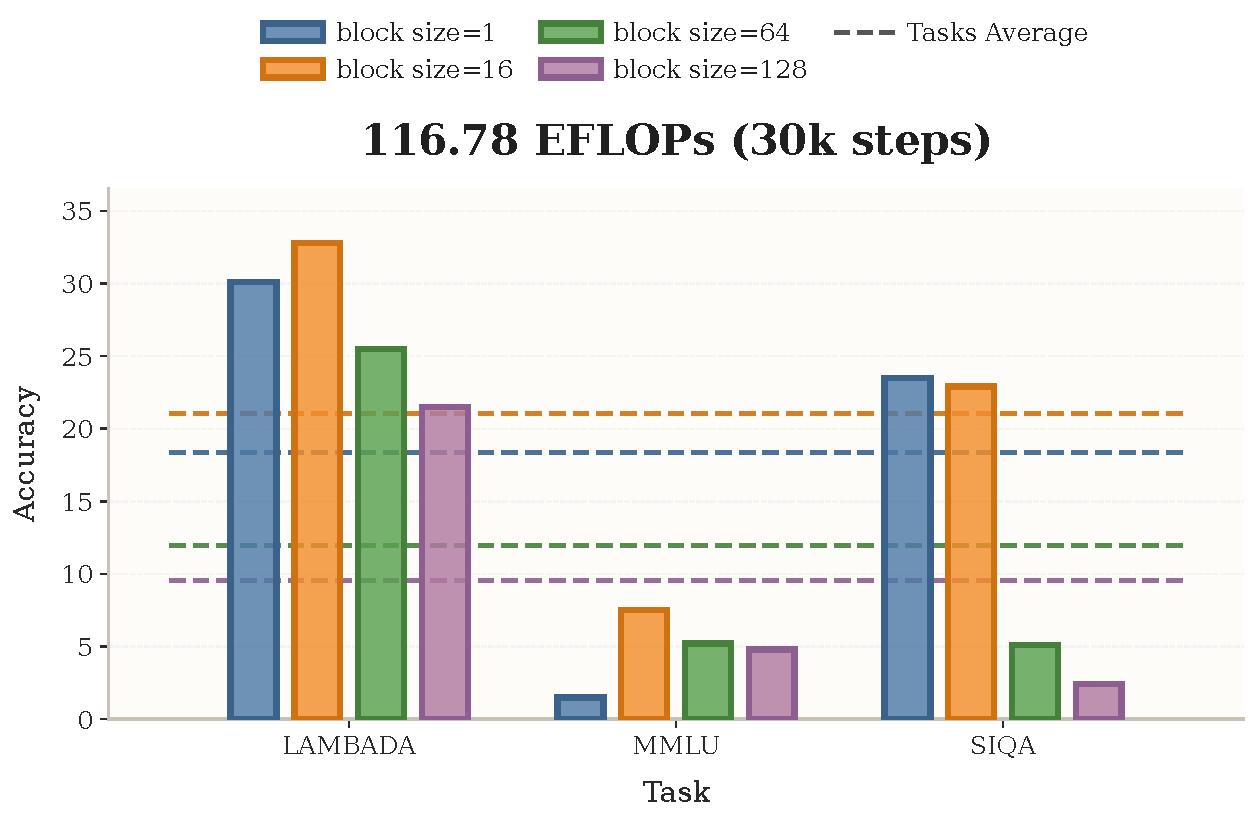
\includegraphics[width=\linewidth]{exp_fig/rq3/dit_block_size/30k.pdf}
        \label{fig:rq3_block_size_30k}
    \end{subfigure}
    \hfill
    \begin{subfigure}[t]{0.49\linewidth}
        \centering
        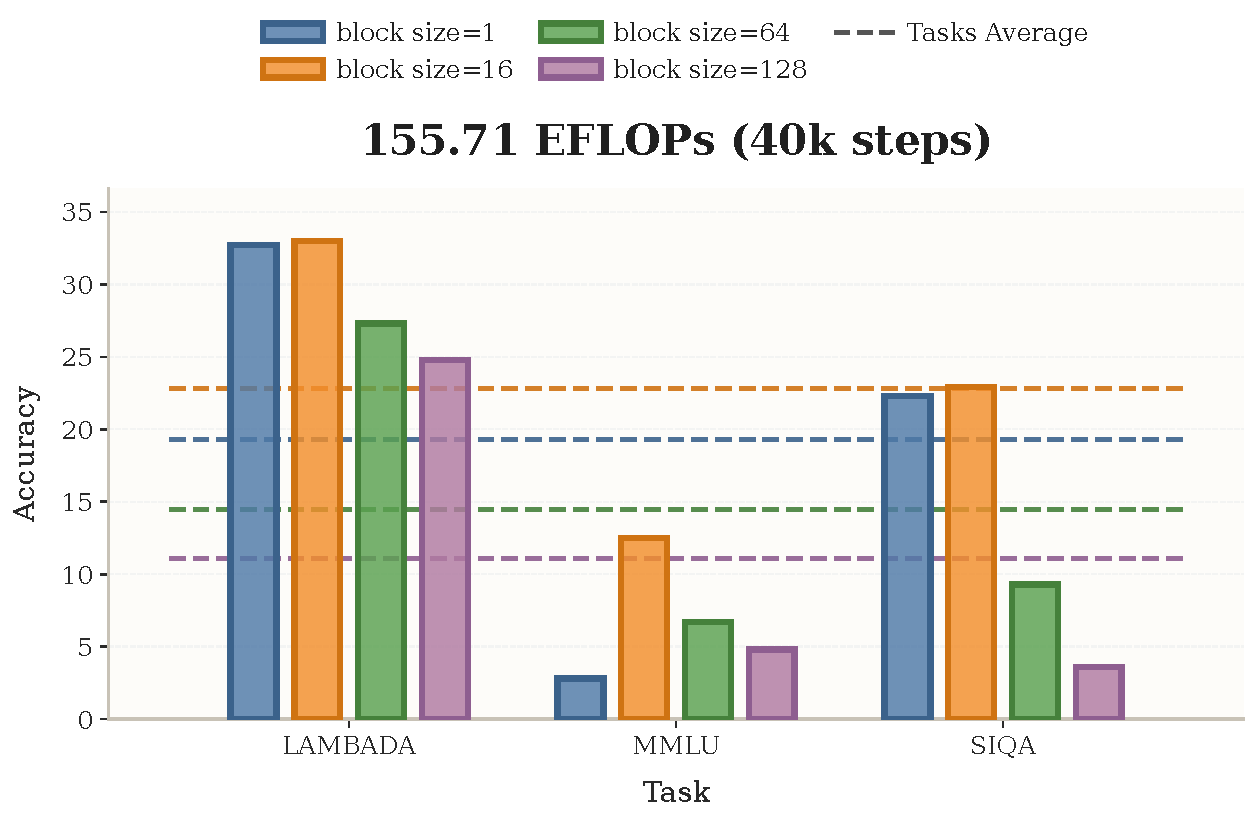
\includegraphics[width=\linewidth]{exp_fig/rq3/dit_block_size/40k.pdf}
        \label{fig:rq3_block_size_40k}
    \end{subfigure}
    \caption{\textbf{Impact of DiT block size.} A moderate block size (especially 16) achieves the best overall performance. Overly large blocks degrade results, while size 1 remains competitive but weaker than 16.}
    \label{fig:rq3_block_size}
\end{figure}

\subsubsection{Training Stage}
\paragraph{DiT Block Size.}As shown in Figure~\ref{fig:rq3_block_size}, all results in this subsection are obtained under the Joint DiT setting: the VAE is initialized from pretrained weights, the VAE and DiT are jointly optimized with the same learning rate, and the training noise schedule uses loc$=1$. We compare four DiT block sizes at two training checkpoints to study how the local processing granularity affects downstream performance. The results show that block size has a clear effect under the current setting, and that a moderate block size works best.

\textbf{Obs. \ding{182} Block size $16$ gives the best overall performance at both checkpoints.}
At both 30K and 40K checkpoints, block size $16$ achieves the highest Task Average in Figure~\ref{fig:rq3_block_size}. It also delivers the strongest or near-strongest results on all three benchmarks, especially on LAMBADA and MMLU. This suggests that, under the current setup, a moderate block size provides a favorable trade-off between local modeling capacity and semantic aggregation.

\textbf{Obs. \ding{183} Larger block sizes are generally less effective under the current setting.}
When the block size is increased from $16$ to $64$ and $128$, performance drops clearly on all three tasks at both checkpoints, with especially visible degradation on SIQA and MMLU. This suggests that overly coarse block partitioning may weaken useful semantic interactions inside the latent sequence. At the same time, since the training noise schedule is fixed to loc$=1$ here, we do not exclude the possibility that different block sizes may favor different noise calibrations.

\textbf{Obs. \ding{184} Block size $1$ is competitive but still weaker than block size $16$.}
Block size $1$ remains a relatively strong baseline and generally outperforms block sizes $64$ and $128$. However, it is still below block size $16$ in Task Average at both checkpoints, and is notably weaker on MMLU. This suggests that fully fine-grained, completely causal processing is not necessarily the optimal way to model text in this setting, and that some degree of local grouping can be beneficial.

Overall, Figure~\ref{fig:rq3_block_size} shows a clear pattern: under the current setting with loc$=1$, DiT block size should be neither too small nor too large. A moderate block size, especially $16$, provides the most effective balance and leads to the best overall performance in the current experiments.

\begin{figure}[t]
    \centering
    \begin{subfigure}[t]{0.49\linewidth}
        \centering
        
\includegraphics[width=\linewidth]{exp_fig/rq3/noise_schedule/line/tasks_avg.pdf}
        \label{fig:rq3_noise_schedule_joint_tasks_avg}
    \end{subfigure}
    \hfill
    \begin{subfigure}[t]{0.49\linewidth}
        \centering
        
\includegraphics[width=\linewidth]{exp_fig/rq3/noise_schedule/line/lambada.pdf}
        \label{fig:rq3_noise_schedule_joint_lambada}
    \end{subfigure}

    \vspace{0.5em}

    \begin{subfigure}[t]{0.49\linewidth}
        \centering
        
\includegraphics[width=\linewidth]{exp_fig/rq3/noise_schedule/line/mmlu.pdf}
        \label{fig:rq3_noise_schedule_joint_mmlu}
    \end{subfigure}
    \hfill
    \begin{subfigure}[t]{0.49\linewidth}
        \centering
        
\includegraphics[width=\linewidth]{exp_fig/rq3/noise_schedule/line/siqa.pdf}
        \label{fig:rq3_noise_schedule_joint_siqa}
    \end{subfigure}
    \caption{\textbf{Noise-schedule ablation.} Across all the tasks, $\mathrm{loc}=1$ gives the strongest overall performance, especially under Joint DiT, while uniform schedules are generally weaker. This suggests that noise-schedule calibration is important and becomes more beneficial when the latent space evolves jointly with DiT.}
    \label{fig:rq3_noise_schedule_joint}
\end{figure}

\paragraph{Noise Schedule. }
As shown in Figures~\ref{fig:rq3_noise_schedule_bar} and~\ref{fig:rq3_noise_schedule_joint}, all results in this subsection are obtained with latent dimension $d=16$ under the Joint DiT setting: the VAE is initialized from pretrained weights, and the VAE and DiT are jointly optimized with the same learning rate. We vary the schedule location parameter to study how noise calibration affects downstream performance, and include Fix VAE curves in Figure~\ref{fig:rq3_noise_schedule_joint} as references. From the information-theoretic analysis in Appendix~\ref{app:noise_schedule_logsnr_fm}, changing the schedule location is not merely changing a training-time heuristic: it effectively shifts the logSNR trajectory of the denoising process, and therefore changes how much semantic information remains available in the latent at different timesteps. The timestep shift formula and visualizations are provided in Appendix~\ref{app:timestep_shift_calc} and~\ref{app:timestep_shift_vis}.

\implicationbox{imp:rq3_noise_schedule}{
If the schedule location shifts the logSNR curve, then it also shifts the effective semantic-information regime seen by the DiT during denoising. Therefore, the best noise schedule is the one whose logSNR trajectory is best aligned with the latent space and the semantic scale to be recovered, rather than a universally fixed timestep parameterization.
}

\textbf{Obs. \ding{182} A moderate schedule location around loc$=1.0$ gives the best overall performance under the current setting.}
Figure~\ref{fig:rq3_noise_schedule_bar} shows that loc$=1.0$ achieves the highest Task Average at both the 30K and 40K checkpoints. It also gives the best or near-best results on the three tasks, with especially clear gains on MMLU and SIQA. From the information-theoretic view developed in Appendix~\ref{app:noise_schedule_logsnr_fm}, this suggests that loc$=1.0$ places the denoising trajectory in a more suitable effective logSNR range for semantic recovery, whereas both smaller and larger shifts move the model away from that regime.

\textbf{Obs. \ding{183} Proper noise calibration is especially important for Joint DiT.}
Figure~\ref{fig:rq3_noise_schedule_joint} further shows that Joint DiT with loc$=1$ is the strongest trainable setting across Task Average, LAMBADA, MMLU, and SIQA, whereas Joint DiT with loc$=0$ or a uniform schedule remains clearly weaker throughout training. Moreover, Joint DiT with loc$=1$ eventually matches or surpasses the corresponding Fix VAE baselines, while the mismatched schedules do not. This indicates that joint latent evolution becomes effective only when the denoising logSNR trajectory is aligned with the semantic structure of the evolving latent space.

\textbf{Obs. \ding{184} The effect of noise schedule should be understood through semantic-information calibration rather than as an isolated hyperparameter effect.}
Appendix~\ref{sec:global_semantic_structure} further implies that schedule location, latent dimension, and VAE logSNR all act on the same core object, namely the effective mutual-information curve of the semantic variable along diffusion time. From this perspective, the sensitivity observed here is not accidental: changing the noise schedule changes where the model spends its denoising capacity on the semantic-information axis. This also helps explain why different latent dimensions, different VAE smoothness settings, and potentially different DiT block sizes need not share the same optimal schedule.

Overall, Figures~\ref{fig:rq3_noise_schedule_bar} and~\ref{fig:rq3_noise_schedule_joint} show that the noise schedule is a key component of the training setup. Under the current Joint DiT setting with $d=16$, a properly calibrated schedule, especially loc$=1.0$, is important not only for stable optimization, but more fundamentally for aligning denoising with the effective semantic-information regime of the latent space. As implied by Eq.~\eqref{eq:main_avg_elbo}, this will further improve the average ELBO and is therefore theoretically well founded.

\begin{figure}[t]
    \centering
    \begin{subfigure}[t]{0.49\linewidth}
        \centering
        
\includegraphics[width=\linewidth]{exp_fig/rq3/noise_schedule/bar/30k.pdf}
        \label{fig:rq3_noise_schedule_bar_30k}
    \end{subfigure}
    \hfill
    \begin{subfigure}[t]{0.49\linewidth}
        \centering
        
\includegraphics[width=\linewidth]{exp_fig/rq3/noise_schedule/bar/40k.pdf}
        \label{fig:rq3_noise_schedule_bar_40k}
    \end{subfigure}
    \caption{\textbf{Noise-schedule comparison at different training checkpoints.} At both checkpoints, $\mathrm{loc}=1.0$ achieves the best Task Average and the most balanced overall performance across tasks. This indicates that the preferred schedule location is stable across training.}
    \label{fig:rq3_noise_schedule_bar}
\end{figure}

\subsubsection{Inference Stage}

\paragraph{Denoising Steps. }
As shown in Figure~\ref{fig:rq3_inferstep}, all results in this subsection are obtained under the Joint DiT setting: the VAE is initialized from pretrained weights, and the VAE and DiT are jointly optimized with the same learning rate. We vary the number of denoising steps at inference time to study the efficiency--performance trade-off. The results show that increasing the number of steps is highly beneficial in the low-step regime, while the gain quickly saturates as the inference budget becomes larger.

\textbf{Obs. \ding{182} Increasing denoising steps yields a clear early improvement.}
From 1--2 steps to 4--8 steps, all tasks improve substantially. The gain is especially large on LAMBADA, while SQuAD, SIQA, and Task Average also increase sharply. This indicates that very few denoising steps are insufficient for stable semantic recovery.

\textbf{Obs. \ding{183} Performance saturates after a moderate number of steps.}
After roughly 16--32 steps, the Task Average becomes nearly flat, and the marginal gain from additional steps is very limited. A similar saturation pattern is also visible on SIQA and SQuAD. This suggests that most useful denoising progress is already completed within a moderate inference budget.

\textbf{Obs. \ding{184} Most of the practical gain is achieved with only 8--10 denoising steps.}
From an efficiency perspective, 8--10 steps already recover most of the final performance. Since our DiT uses a block size of 16, this means 16 tokens can be generated with only 8--10 sequential denoising iterations, corresponding to an idealized 1.6--2.0$\times$ reduction in sequential generation depth compared with AR decoding.

\begin{figure}[t]
    \centering
    \begin{subfigure}[t]{0.47\columnwidth}
        \centering
        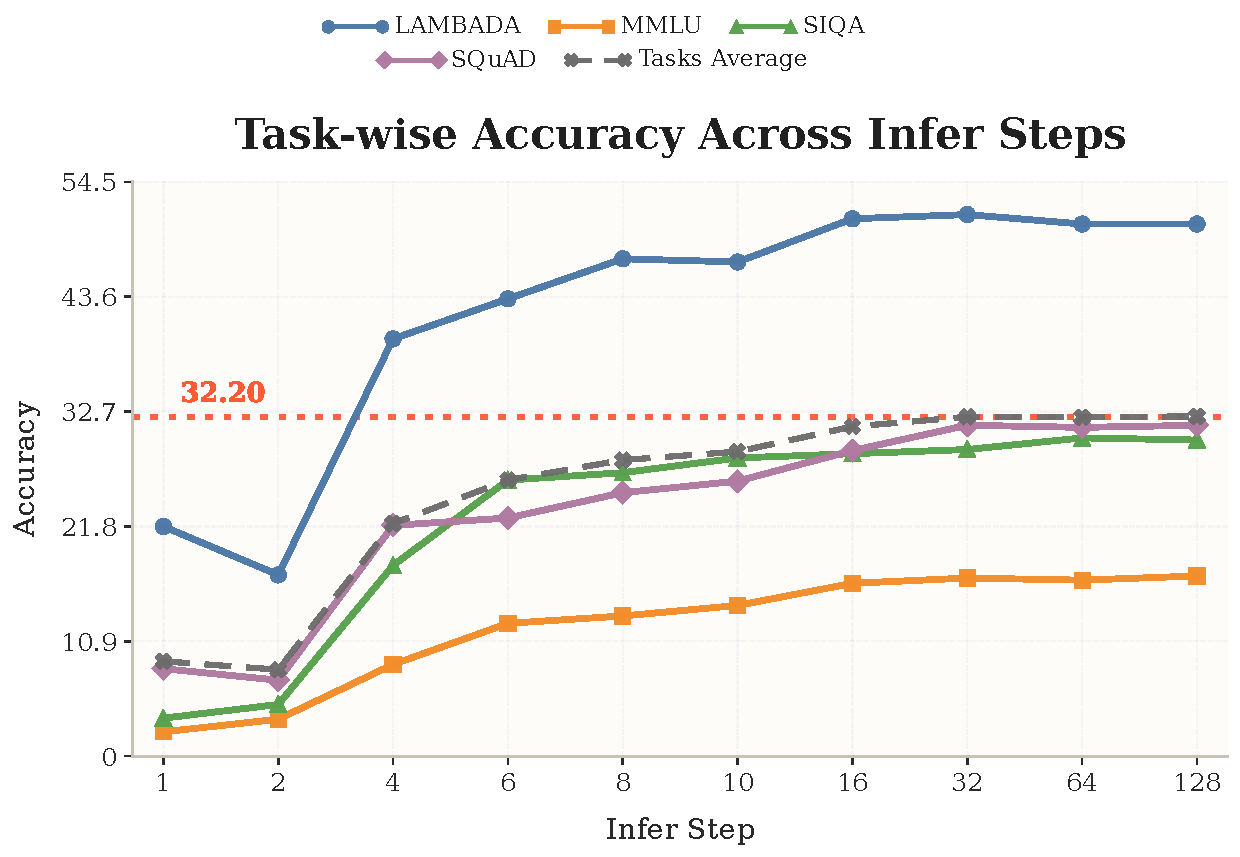
\includegraphics[width=\linewidth]{exp_fig/rq3/inferstep/task_vs_inferstep.pdf}
        \caption{\textbf{Impact of denoising steps}}
        \label{fig:rq3_inferstep}
    \end{subfigure}
    \hfill
    \begin{subfigure}[t]{0.52\columnwidth}
        \centering
        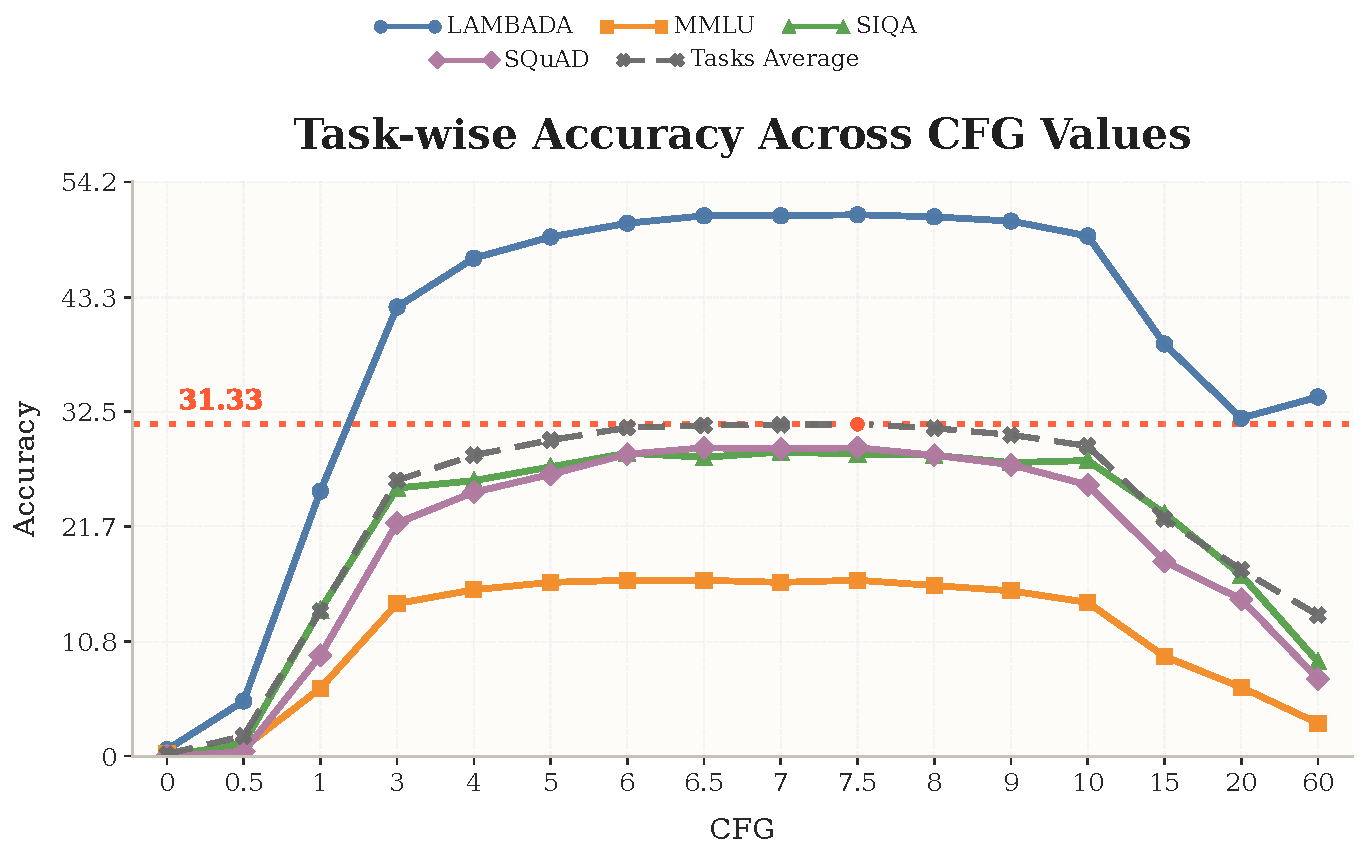
\includegraphics[width=\linewidth]{exp_fig/rq3/cfg/task_vs_cfg.pdf}
        \caption{\textbf{Impact of CFG scales}}
        \label{fig:rq3_cfg}
    \end{subfigure}
    \caption{\textbf{Impact of inference-time hyperparameters.} Increasing denoising steps brings clear early gains but quickly saturates, while a moderate CFG value achieves the best overall performance.}
    \label{fig:rq3_infer_cfg}
\end{figure}

Overall, Figure~\ref{fig:rq3_inferstep} shows that denoising steps are important, but more is not always better. Under the Joint DiT setting, a moderate number of inference steps, around 10--32, already provides a strong trade-off between accuracy and efficiency.

\paragraph{Classifier-Free Guidance (CFG) Scales. }
As shown in Figure~\ref{fig:rq3_cfg}, all results in this subsection are obtained under the Joint DiT setting: the VAE is initialized from pretrained weights, and the VAE and DiT are jointly optimized with the same learning rate. We vary the Classifier-Free Guidance (CFG) scale at inference time to study how guidance strength affects downstream performance. The results show a clear non-monotonic pattern: increasing CFG is helpful at first, but overly large values significantly hurt performance.

\textbf{Obs. \ding{182} A moderate CFG scale gives the best overall performance.}
The Task Average rises rapidly as CFG increases from $0$ to around $3$--$6$, and then stays near its best region for a moderate range of values. This indicates that an appropriate amount of guidance substantially improves conditional denoising and semantic recovery.

\textbf{Obs. \ding{183} Excessive guidance leads to clear degradation.}
After the moderate optimum region, all task curves begin to decline as CFG becomes larger. The drop is especially pronounced beyond CFG $\approx 10$, and becomes severe at very large values such as $20$ and $60$. This shows that overly strong guidance distorts the denoising trajectory rather than improving it.

Overall, Figure~\ref{fig:rq3_cfg} shows that CFG is an important inference-time hyperparameter. Under the Joint DiT setting, a moderate CFG scale provides the best trade-off, while both weak guidance and excessive guidance lead to inferior results.

\subsection{Comparison of Scaling Performance (RQ4)}
\label{exp:rq4}

\begin{figure}[t]
    \centering
    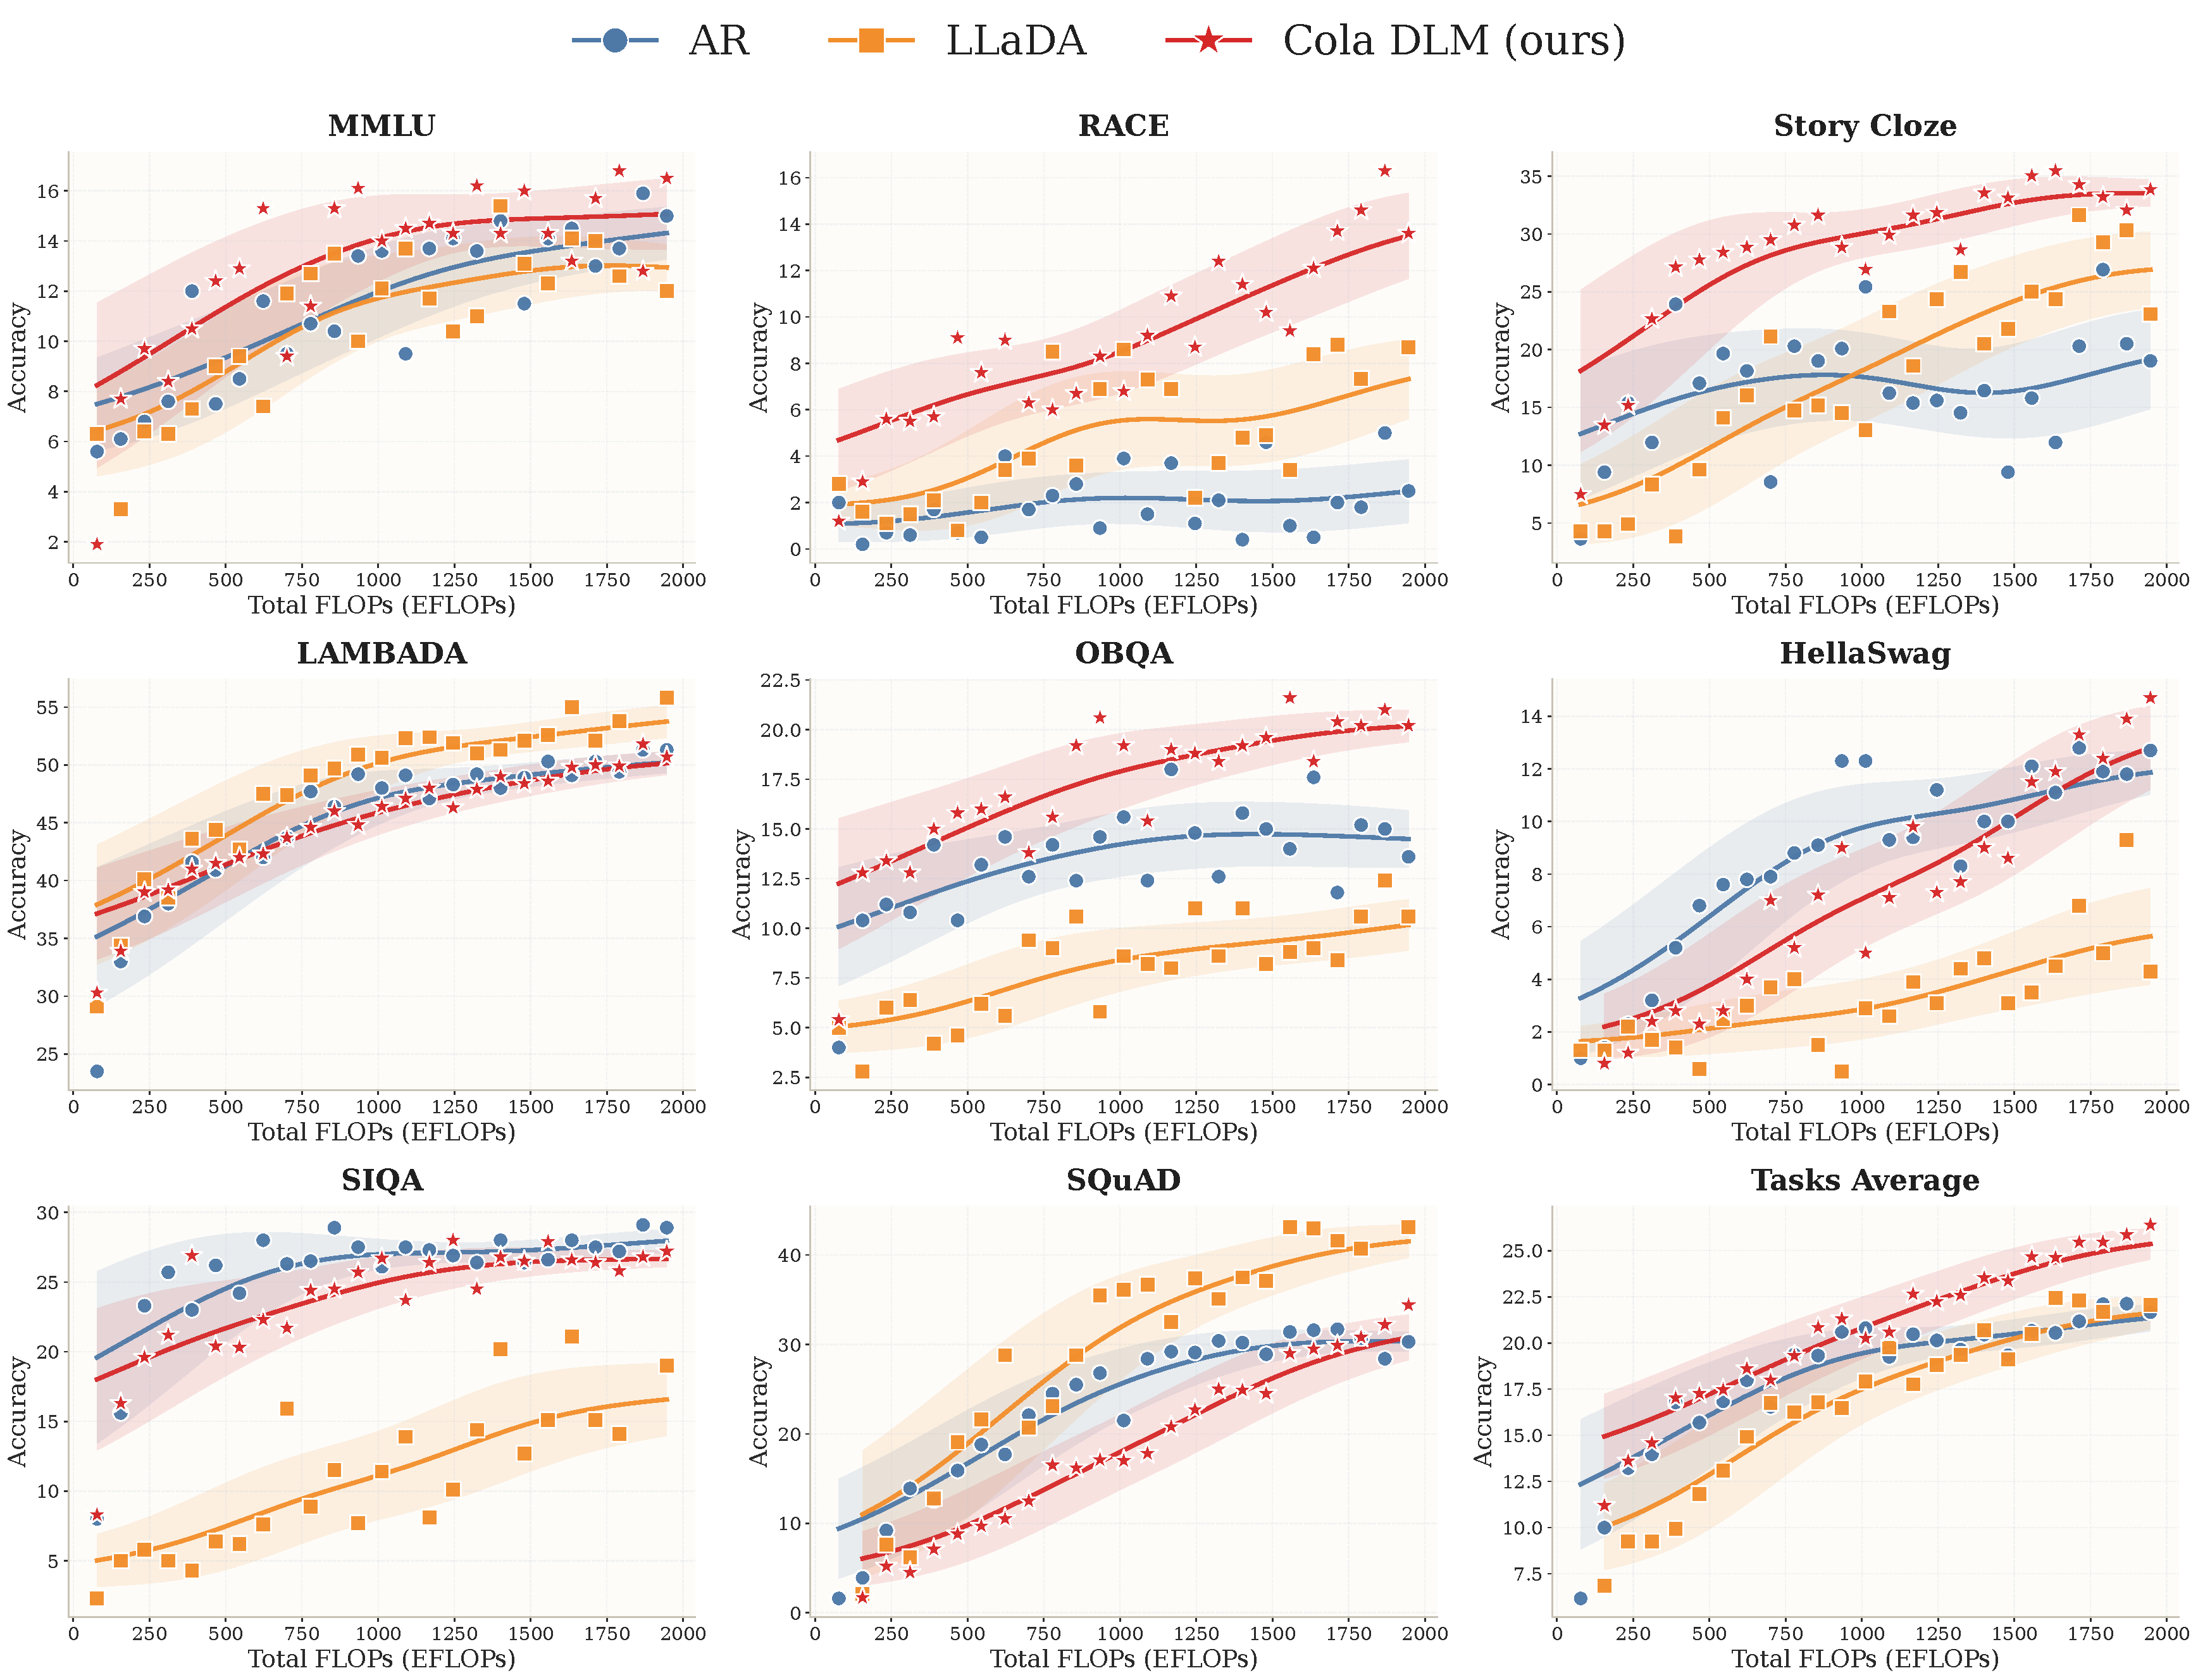
\includegraphics[width=1\textwidth]{exp_fig/rq4/group_tasks.pdf}
    \caption{\textbf{Overall scaling performance under a unified few-shot generative evaluation protocol.} Across eight benchmarks and Task Average, \method exhibits strong scaling dynamics, ultimately reaching the best average performance. It should be noted that the lower absolute accuracy observed on specific multiple-choice tasks is an anticipated consequence of the rigorous generative evaluation paradigm; nevertheless, the underlying scaling trends are robustly preserved. These findings imply that continuous latent prior modeling possesses significant scaling potential, rendering the current performance a conservative measure of its true capacity.}
    \label{fig:scaling_exp_fig}
\end{figure}

In this section, we compare the scaling behavior of \method with strictly matched AR and LLaDA baselines under the best configuration identified by the previous tuning experiments. Specifically, \method uses latent dimension $d=16$, block size $16$, joint VAE--DiT training with a VAE/DiT learning-rate ratio of $1$, BERT loss, and a logit-normal training noise schedule with $\mathrm{loc}=1$; at inference time, we use $16$ denoising steps and CFG $=7$. The AR and LLaDA baselines are matched in scale, with the non-embedding backbone controlled at $1.8$B parameters, and LLaDA uses a denoising length equal to the generation length during inference.

It is also worth noting that the absolute scores in Figure~\ref{fig:scaling_exp_fig} are relatively low mainly on the multiple-choice benchmarks. This is because, for a fair comparison, all models are evaluated under a unified few-shot generative protocol rather than standard likelihood-based classification: LAMBADA and SQuAD are evaluated as generative tasks, while the remaining benchmarks are multiple-choice tasks but are also cast into few-shot generation. As discussed in Section~\ref{dis:ppl}, likelihood estimation can be substantially misaligned with the actual generation quality of \method. Therefore, although the absolute values on multiple-choice tasks are lower than those in conventional discriminative evaluation, the relative scaling trends remain informative and fair under this fully matched protocol.

As shown in Figure~\ref{fig:scaling_exp_fig}, \method exhibits strong overall scaling behavior, with increasingly encouraging gains as the compute budget grows.

\textbf{Obs. \ding{182} \method shows one of the strongest overall scaling trends.}
On Task Average, \method improves steadily across the full compute range and reaches the best final performance. AR remains competitive at smaller budgets, and LLaDA also shows clear early gains, but the curve of \method rises more persistently toward the high-compute regime. This suggests that \method already exhibits highly competitive, and at larger budgets stronger, scaling potential under the current matched setting.

\textbf{Obs. \ding{183} The scaling advantage of \method is especially clear on reasoning-intensive and global-semantic tasks.}
On MMLU, RACE, Story Cloze, and OBQA, \method maintains a strong upward trend and achieves the best or near-best performance across a wide compute range. The gains are particularly visible at medium-to-large budgets, indicating that continuous latent prior modeling is well suited to tasks that rely more on global semantic organization and holistic answer formation.

\textbf{Obs. \ding{184} On generative tasks, \method also shows encouraging scaling behavior.}
For LAMBADA and SQuAD, the scaling trends remain clear under the unified generative evaluation protocol. On LAMBADA, \method improves steadily with compute and remains close to AR at larger budgets, while SQuAD shows a particularly clear gain with scale, where \method eventually surpasses AR and continues to approach the strong performance region of LLaDA. These results suggest that, on generation-oriented evaluation, \method already demonstrates scaling behavior comparable to strong baselines, with encouraging headroom as compute increases.

\textbf{Obs. \ding{185} The current result is a conservative estimate of the scaling potential of \method.}
The present comparison is conducted under a relatively conservative configuration of \method. Earlier ablations already show that increasing the latent dimension from $16$ to $128$ can improve semantic capacity, and the analysis of logSNR also suggests that the current setting still leaves additional room for scaling. Therefore, Figure~\ref{fig:scaling_exp_fig} should be viewed as evidence that \method already scales well under a restrained setting, rather than as the upper bound of its capability.

Overall, Figure~\ref{fig:scaling_exp_fig} supports a consistent conclusion: under a strictly matched comparison and a unified generative evaluation protocol, \method exhibits scaling behavior that is fully competitive with strong AR and diffusion-based baselines, and on several tasks already shows particularly encouraging late-stage gains. Together with the remaining optimization headroom in latent-space design, these results provide supportive evidence that continuous latent prior modeling is a promising scaling direction for language modeling.

